% !TeX root = ../main.tex
% Add the above to each chapter to make compiling the PDF easier in some editors.
\graphicspath{{./figures/ch4/}}

\chapter{Simulation}\label{chapter:simulation}

To find out how the HPB format influences efficiency and revenue in comparison to the SMRA, I ran several simulations based on the findings in the previous chapter. For the bidders to act as agents in the auction simulations, they need a strategy and a suitable selection heuristic to model their behaviour and thus to place bids. In this chapter I will at first give an overview of the structure of the implementation, followed by a further description of the simulation process by defining the setup as well as the strategy and the selector model. Afterwards, I will present the findings of the experiment.

\section{Structure of the Project}
In order to run the simulations I extended an existing project from the university chair. In this project, an abstract structure on how to run auction simulations was given by an already defined software architecture. \autoref{fig:structure-sim} visualises the structure I used for my experiment. The whole project was implemented in Python.

As can be seen from the visualisation, a main \textbf{Auction} object exists, that has an own \textbf{AuctionFormat} which specifies the auction characteristics and the procedure, as well as a collection of agents participating. Every \textbf{Agent} possesses a bidding \textbf{Strategy} which in turn holds a \textbf{Selector}. The latter computes optimal bidding vectors based on the chosen selector model (e.g. a naive exhaust approach by iterating over each possible bid). Then the strategy translates these into according actions like submitting a bid based on the selector's result or calling a waiver to exclude the agent from bidding in the current round. The strategy class realises this by comparing the payoff $ \pi_{combination} $ of different combinations, where payoff is defined as a \textit{quasilinear utility function} by subtracting the prices $ p(combination) $ a bidder has to pay from the bidder's valuation $ v(combination) $ for a certain bidding combination.

\begin{equation}
	\centering
	\pi_{combination} = v(combination) - p(combination)
	\label{eq:payoff}
\end{equation}

The valuation $ v(combination) $ can be obtained by the strategy class using its \textbf{ValueModel}. This model has access to the \textbf{ItemStructure}, which holds the \textbf{Items} of the auction as well as possible packages, mapping (e.g. to frequency bands), or hierarchies. Before submitting a bid, the action gets validated by the \textbf{BidderInfo} class (e.g. to check if spectrum cap instructions were followed). After each successful round, the important information like \textit{payments, prices}, and the current \textit{allocation} are saved in the \textbf{RoundInfo}.

\begin{figure}[h]
	\centering
	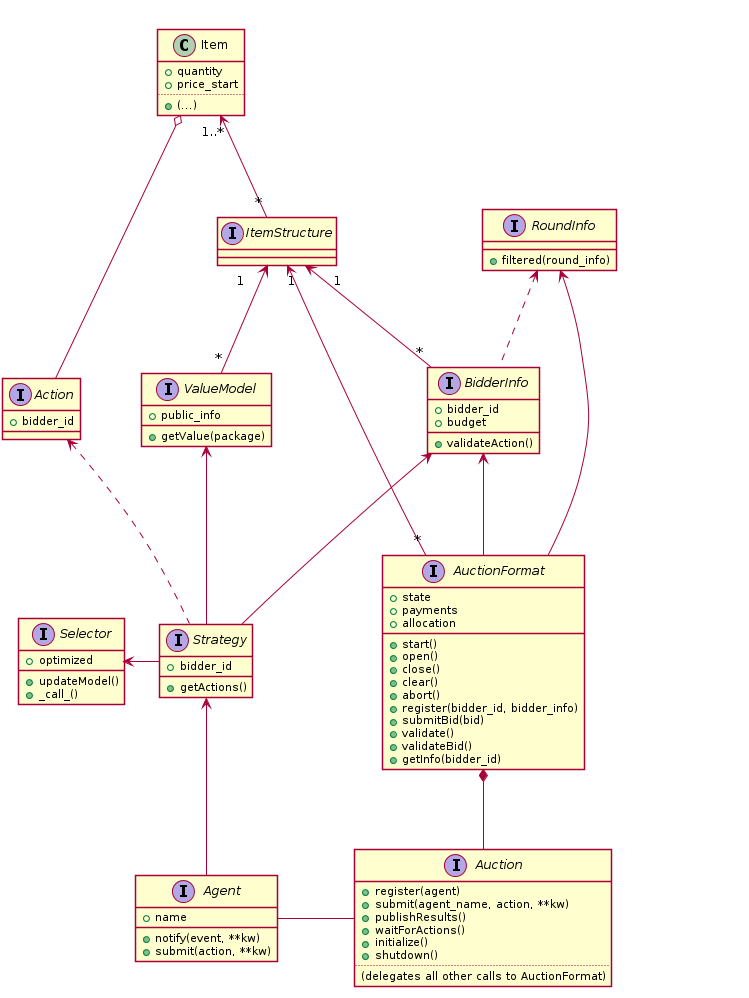
\includegraphics[scale=0.4]{structure.png}
	\caption{Structure of the simulation implementation} \label{fig:structure-sim}
\end{figure}

To simulate the auctions I had to extend the existing auction formats for SMRA and HPB. Making it possible to fill them with the specific characteristics of the German auction. In particular, this included implementing the spectrum cap of three blocks in the 900 MHz band and extending mechanisms in the HPB format. Also, I needed to implement the mathematical formulation of the value model (see \autoref{subsection:value-model}) as well as the specific selector model, which is based on the value model. Furthermore, I implemented a sealed bid model to calculate the optimal allocation needed to compare the two auction formats.


\section{The Simulation Process}
As stated in the previous section, in order to run the simulations based on the information and data of the German Auction I needed to extend and further develop the existing project. In this section I will describe the set-up of the auctions (e.g. the items and hierarchies used) as well as the implementation of the value, strategy and selector model.

\subsection{Auction Set-Up}
As discussed in the Value Model section, the simulation concentrated on the 700, 900 and 1800 MHz frequency bands, which include a total of 23 items. Each bidder was able to bid on every item and item combination. For the first round, the starting prices were appointed according to the official definition of the German Auction \cite{Bundesnetzagentur2015} as provided in \autoref{tbl:start-parms}.

\begin{table}[h]
	\centering
	\begin{tabular}{|c|c|c|c|}
		\hline
		\textbf{block} & \textbf{quantity} & \textbf{\begin{tabular}[c]{@{}c@{}}starting\\ price\end{tabular}} & \textbf{\begin{tabular}[c]{@{}c@{}}eligibility\\ points\end{tabular}} \\ \hline
		700 MHz        & 6                 & EUR 75 mn                                                         & 2                                                                     \\ \hline
		900 MHz        & 7                 & EUR 75 mn                                                         & 2                                                                     \\ \hline
		1800 MHz       & 10                & EUR 37.5 mn                                                       & 2                                                                     \\ \hline
	\end{tabular}
	\caption{Starting parameters for the items in the auction}
	\label{tbl:start-parms}
\end{table}
The activity level was chosen to be 65\% of the eligibility points held by each bidder in every round. This is the activity level chosen in the first phase of the German Auction. As no mathematical progression rule for the phase shifts exists, because they are decided by the auction moderator \cite{Bundesnetzagentur2015}, the activity level stayed the same throughout the auction simulations. 
Furthermore, the exposure ratio (the degree to which a bidder can overbid the valuation of an item) was set very high, practically eliminating exposure. This decision was made, as deriving a fitting exposure ratio for the simulation was out of the scope of this thesis. I will discuss the implications in \autoref{chapter:conclusion}. 

As HPB makes use of pre-defined packaging of items using a tree structure, I needed to develop a useful item hierarchy to be used in the simulation. To show how the hierarchy affects the bidding and thus efficiency and revenue, I created two slightly different hierarchy models. As the 900 MHz band had a spectrum cap, the bidders were limited on how many items they can acquire (here: maximum of three blocks). The other bands had no such limitations, thus each bidder would try to acquire the most items possible under the constraints of item valuations and maximizing payoff. To research the impact of the hierarchies on the bidding behaviour, I devised two different hierarchies that had different pre-packaging in the 900 MHz band, because bidders were only allowed to acquire up to three blocks, a combination that had super-additive valuation for the bidders (\autoref{subsection:value-model}) and I assumed the competition to be high in this band. \autoref{fig:hpb-hierarchy-competition} shows the item hierarchy called $ H_{competition} $, where one package of three items (reflecting a desired bundling) exists in the structure. The hierarchy is called "competition" as only one of the desired bundling exists. 

\begin{figure}[]
	\centering
	\usetikzlibrary{shapes}

\begin{adjustbox}{valign=t}
	\centering
	\begin{forest}
		rounded/.style={ellipse, draw}
		[{\textbf{700 MHz}}, for tree=rounded
		[{A, B}
		[A][B]]
		[{C, D}
		[C][D]]
		[{E, F}
		[E][F]]]
	\end{forest}
\end{adjustbox} \quad
\begin{adjustbox}{valign=t}
	\begin{forest}
		rounded/.style={ellipse, draw}
		[{\textbf{900 MHz}}, for tree=rounded
		[{A, B}
		[A][B]]
		[{C, D}
		[C][D]]
		[{E, F, G}, red
		[E][F][G]]]
	\end{forest}
\end{adjustbox}
	\begin{adjustbox}{valign=t}
	\begin{forest}
		rounded/.style={ellipse, draw}
		[{\textbf{1800 MHz}}, for tree=rounded
		[{A, B, C, D}, red
		[A][B][C][D]]
		[{E, F, G, H}, red
		[E][F][G][H]]
		[{I, J}
		[I][J]]]
	\end{forest}
\end{adjustbox}
	\caption{HPB Hierarchy "Competition", packages with bonus in red}
	\label{fig:hpb-hierarchy-competition}
\end{figure}

As the 900 MHz band consists of seven items, it has enough items for incorporating two bundles of three items each. I assumed that following the formulation and the bonuses of the value model (see \autoref{subsection:value-model}) at least two bidders will try to acquire bonus enabling packages. This is what $ H_{VM} $ in \autoref{fig:hpb-hierarchy-vm-predict} incorporates. 
Note, that bidders were still able to gain super-additive valuation by bidding on single items (in different packages) and still be able to successfully secure three items in the 900 MHz band. In the HPB simulation, the advantage for bidders was that they could bid on packages, signalling an interest in a certain item combination. When bidding on the package, the bidder either acquires all the items in its desired packaging or none, thus resulting in a reduced exposure risk for the bidders as it prevents him from potentially bidding above an item's valuation in order to realise a certain item combination.

\begin{figure}[]
	\centering
	\usetikzlibrary{shapes}

\begin{adjustbox}{valign=t}
	\centering
	\begin{forest}
		rounded/.style={ellipse, draw}
		[{\textbf{700 MHz}}, for tree=rounded
		[{A, B}
		[A][B]]
		[{C, D}
		[C][D]]
		[{E, F}
		[E][F]]]
	\end{forest}
\end{adjustbox} \quad
\begin{adjustbox}{valign=t}
	\begin{forest}
		rounded/.style={ellipse, draw}
		[{\textbf{900 MHz}}, for tree=rounded
		[{A, B, C}, red
		[A][B][C]]
		[{D, E, F}, red
		[D][E][F]]
		[{G}
		[G]]]
	\end{forest}
\end{adjustbox}
	\begin{adjustbox}{valign=t}
	\begin{forest}
		rounded/.style={ellipse, draw}
		[{\textbf{1800 MHz}}, for tree=rounded
		[{A, B, C, D}, red
		[A][B][C][D]]
		[{E, F, G, H}, red
		[E][F][G][H]]
		[{I, J}
		[I][J]]]
	\end{forest}
\end{adjustbox}
	\caption{HPB Hierarchy "VM Prediction", packages with bonus in red}
	\label{fig:hpb-hierarchy-vm-predict}
\end{figure}

\subsection{Strategy and Selector Model}
In the simulation, the participating agents needed to emulate a certain bidding behaviour. This is realised by the strategy model. In this experiment, the bidders followed a \textbf{straightforward bidding} behaviour, essentially meaning that they always bid according to the minimum prices in each round \cite[p. 270.]{Milgrom2000}. This can be described as a function $ p(I) $ that returns the bidding price of an item according to minimum prices, where $ \beta $ is the current bid price \cite[p. 6 ff.]{Wellman2008}.

\begin{equation}
	p(I) = 
		\begin{cases}
			\beta & \text{if item is already won} \\  
			\beta + increment & \text{otherwise}
		\end{cases} 
		\label{eq:sb-prices}
\end{equation}

The straightforward bidding is also called \textit{"myopic best response"} \cite{Brooks2000}. Additionally, the strategy used in the simulation is payoff maximizing.
 
As explained in the section above, value models return the valuation of certain item combinations and selectors return optimal bidding vectors $ \vec{\theta} $. The strategy model translates the results into an according action, e.g. a bid based on a payoff maximizing strategy.  

One could argue that once the simulations are run on a computer, finding the best bidding combination should be done via an exhaustive iteration over every single possible combination. However, using this approach showed to be an ineffective use of time and to be computationally expensive. The number of items in the simulation was 23. Lining up all the items in fixed order and using a binary vector to display if each respective item should be included into a bid creates the vector $ \vec{\theta} \in \{0,1\}^{23} $. With simple combinatorics it can be deduced, that computing every possible allocation takes $ 2^{23} \approx 8.388 \times 10^{6} $ iterations. Remembering that 700 MHz had 6 blocks, 900 MHz 7 blocks and 1800 MHz 10 blocks and taking into account, that bidders were only allowed to acquire up to three blocks in the 900 MHz band, the number of iteration can be reduced to $$ 2^6 * \sum_{i=1}^{3} \binom{n}{k} * 2^{10} = 2^6 * (2^6 - 1) * 2^{10} = 2^{16} * (2^6-1) = 2^{22} - 2^{16} \approx 4.1 \times 10^6 $$
Due to the current implementation in the project, this has to be done twice for each of the three bidders, requiring an amount of $ 2 \times 3 \times 2^{22} - 2^{16} \approx 25.1 \times 10^{6} $ computation steps each auction round.   
Clearly, a different approach was needed to select the optimal bidding vector. 

Instead, a \textbf{mixed integer linear program} (MILP) %TODO abbr
was used to compute the optimized bidding vector $ \vec{\theta} $. For that, I extended existing code for an additive payoff selector from the main project and added the specific bonuses and caps to the LP. Additionally, the bidders had to incorporate bidding on packages, when the payoff for single items and package bids were the same. This behaviour was integrated by adding a \textit{very small} bonus for using packages to the objective function (Epsilon-Method). When a bidder would bid on a package, the payoff would be marginally higher than when bidding on the single items, but by only a very small number which does not affect the overall allocation. The MILP formulation is very similar to the one in \autoref{subsection:meth-evaluation}, but this time only computes the best allocation for a single bidder. Also, the bidder's objective function was extended by the small "bidding-on-HPB-package-bonus", so that the selector MILP can take the existing package hierarchy into account. So for each super-additive package $ p \in Hierarchy $ the objective function increases by a very small amount (in comparison to the sum of all the valuations) if the package was bid on. This leads to the following MILP formulation, where $ Hierarchy_{900}, Hierarchy_{1800} \in Hierarchy $ are the respective subsets of packages in the 900 and 1800 MHz bands and $ Hierarchy_{900bonus} \in Hierarchy_{900}, Hierarchy_{1800bonus} \in Hierarchy_{1800} $ the respective subsets with bonus packages. Additionally, $ bonusV_{900} $ and $ bonusV_{1800} $ stand for the bidder's valuation of the bonuses, they correspond to the $ V_{MNO}^{900_3} $ and $ V_{MNO}^{1800_4} $ from \autoref{subsection:value-model}  where $ MNO $ equals the respective bidder.

\begin{align*}
	& {\text{maximize}}
	& & \sum_{i \in Items} ass_{i} * V_{i} + b_{900} * bonusV_{900}  + b_{1800} *bonusV_{1800} \\ 
	& & & + \varepsilon * \Bigg[ \sum_{p \in Hierarchy_{900bonus}} m_p + \sum_{p \in Hierarchy_{1800bonus}} m_p \Bigg] \\
	& \text{subject to}
	& & \sum_{i \in Items_{900}}  ass_{i}  \geq 3 *  b_{900} \tag{\textit{Bonus in 900 MHz}}  \\
	&&& \sum_{i \in Items_{1800}}  ass_{i}  \geq 4 *  b_{1800} \tag{\textit{Bonus in 1800 MHz}} \\
	&&& \sum_{i \in Items_{900}}  ass_{i}  \leq 3 \tag{\textit{Caps in 900 MHz}} \\
	&&& \sum_{i \in p} ass_i \geq |p| * m_p \quad \forall p \in Hierarchy_{900bonus} \cup Hierarchy_{1800bonus} \tag{\textit{Preemptive bundle selection}} \\
	& \text{where}
	& & V_{i}, bonusV_{900}, bonusV_{1800} \in \mathbb{N}, \quad \forall i \in Items \\
	&&& ass_{i}, b_{900}, b_{1800} \in \{0,1\} \\
	&&& m_p \in \{0,1\}, \quad \forall p \in Hierarchy
\end{align*}\label{eq:selector-lp}

\section{Results}
Now, with the project incorporating all the characteristics of the German Auction I was able to simulate the SMRA and HPB auctions. To research the sensitivity of efficiency and revenue towards the change of the set-up parameters I ran simulations iterating over sequences of the parameters $ \beta_{900}, \beta_{1800} $ and $ s_{DT}, s_{VOD} $ for both Hierarchies $ H_{competition}, H_{vm-prediction} $. Because of the high number of possible parameter combinations I will focus on the most important results below. To answer the question \textit{"How well does HPB perform in comparison to SMRA in the context of the German Auction?"}, my analysis was mainly guided by the following questions:

\begin{itemize}
	\item How sensitive are \textit{efficiency} and \textit{revenue} to \textit{bonus valuations}?
	\item What is the impact of the \textit{HPB hierarchy} on both metrics?
	\item How does \textit{efficiency} and \textit{revenue} change in relation to the environment of \textit{bidder strengths}?
\end{itemize}

\subsection{Efficiency of the Formats}\label{subsection:eff-formats}
A \textit{"well performing"} auction results in a (near-)optimal allocation of the bidding items to the bidders, meaning reaching a high efficiency is desired. As described in \autoref{subsection:meth-evaluation}, efficiency is described as the ratio of the total welfare achieved in relation to the optimal welfare, which is calculated by running a sealed-bid model on the parameters. Therefore, the efficiency of the sealed-bid model is always equal to one and the other formats are judged on this basis.

\begin{figure}[h]
	\centering
	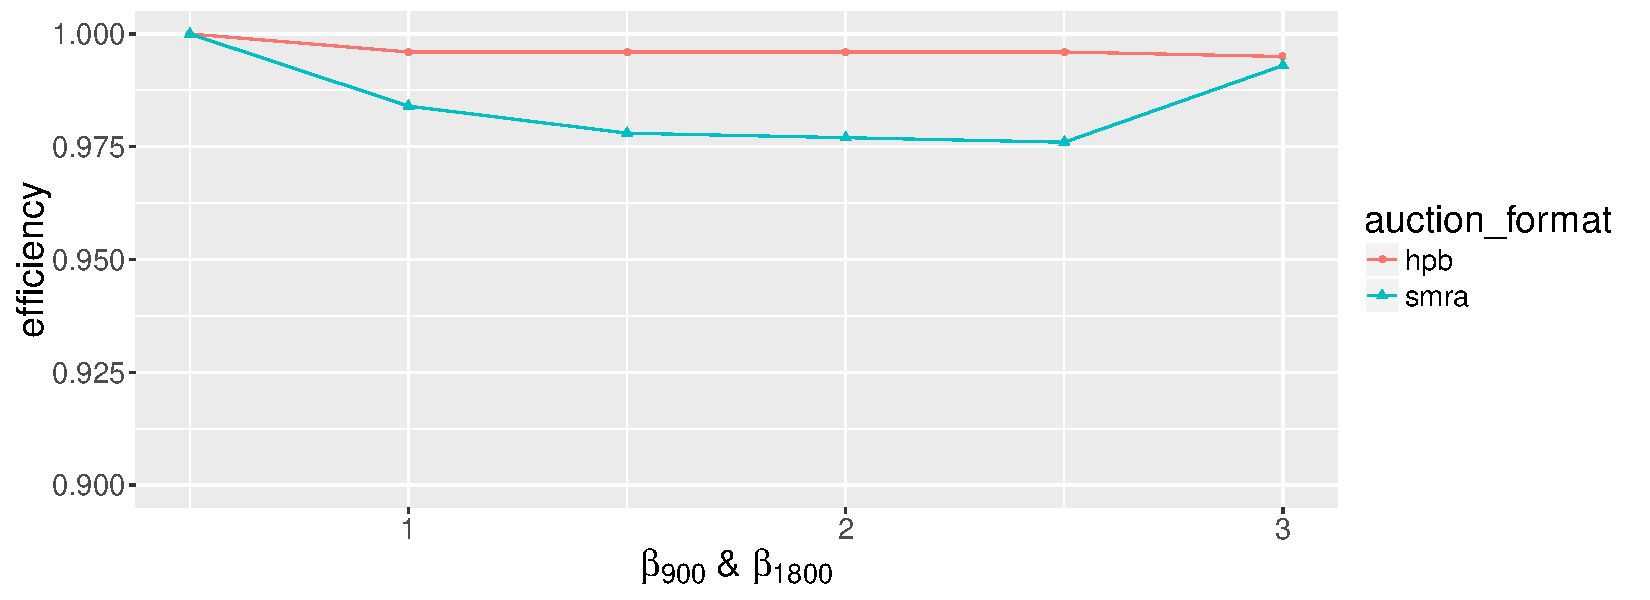
\includegraphics[scale=0.5]{eff_both_betas_moving.pdf}
	\caption{Sensitivity of efficiency against $ \beta_{900} = \beta_{1800} $ in $ H_{competition} $} \label{fig:eff-both-beta-mov}
	
	\vspace*{\floatsep}
	
	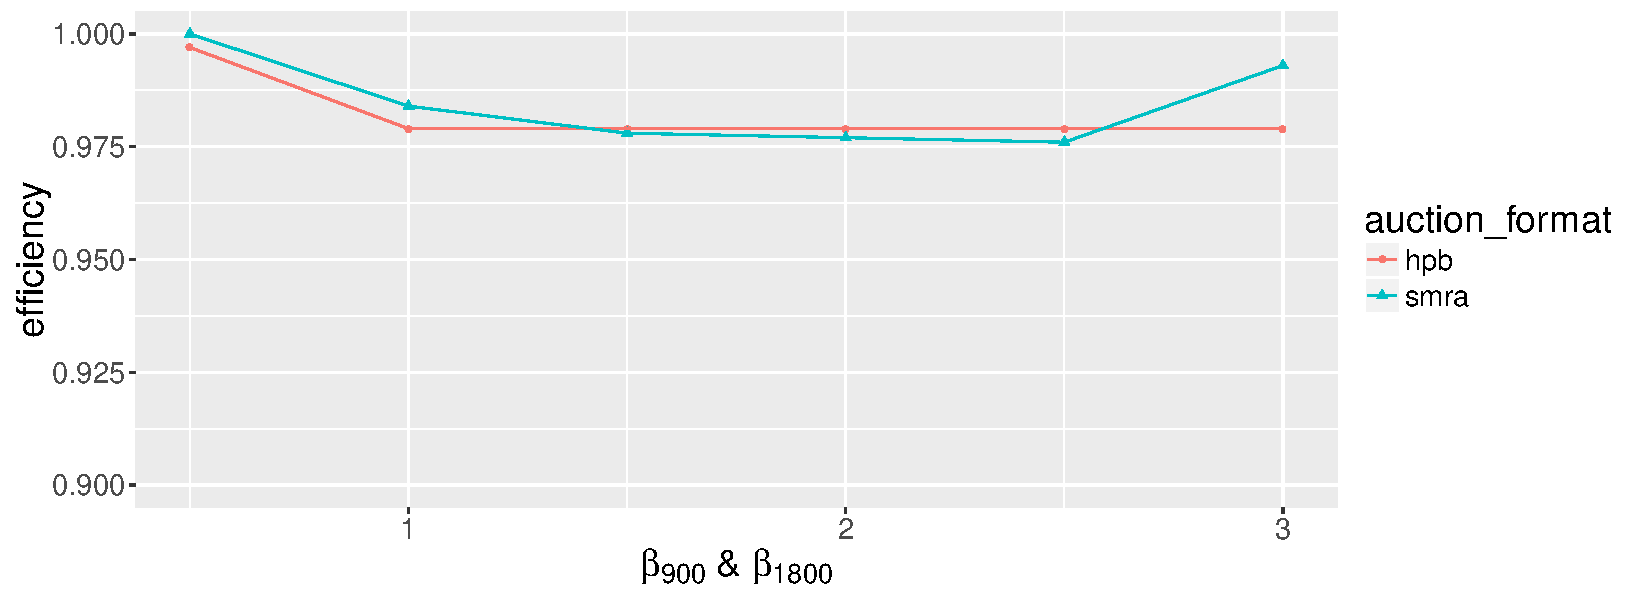
\includegraphics[scale=0.5]{eff_both_betas_moving_VMP.pdf}
	\caption{Sensitivity of efficiency against $ \beta_{900} = \beta_{1800} $ in $ H_{vm-prediction} $} \label{fig:eff-both-beta-mov-vmp}
\end{figure}

%\paragraph{The influence of bonus valuations and hierarchies.}
When running simulations iterating over the bonuses valuations, differences between both hierarchies became clear. \autoref{fig:eff-both-beta-mov} shows the development of efficiency in relation to the bonuses valuations in the $ H_{competition} $ hierarchy and \autoref{fig:eff-both-beta-mov-vmp} for $ H_{vm-prediction} $ respectively. Despite the fact that the efficiency levels of HPB showed to be more stable than SMRA, there were differences in the results between the two hierarchies. 
In $ H_{competition} $ HPB showed to be superior to SMRA with $ HPB \succ SMRA $. Also, HPB showed to be much more stable in resulting in a high efficiency level, which was near-optimal. In comparison, the overall allocation in SMRA seems to be more susceptible to the bonuses valuations, but still resulting in a high efficiency.

From the data it seems that in HPB the valuation of the bonus inducing packages has little effect on the overall allocation and efficiency of the auction, making it a versatile tool to auction items with such characteristics. But the correct choice of the structure appears to be an important question. The findings indicate, that a competitive HPB hierarchy might help in reaching a better overall allocation in comparison SMRA. But this needs to be verified by further experiments (see \autoref{chapter:conclusion}). 

%\begin{figure}[h]
%	\centering
%	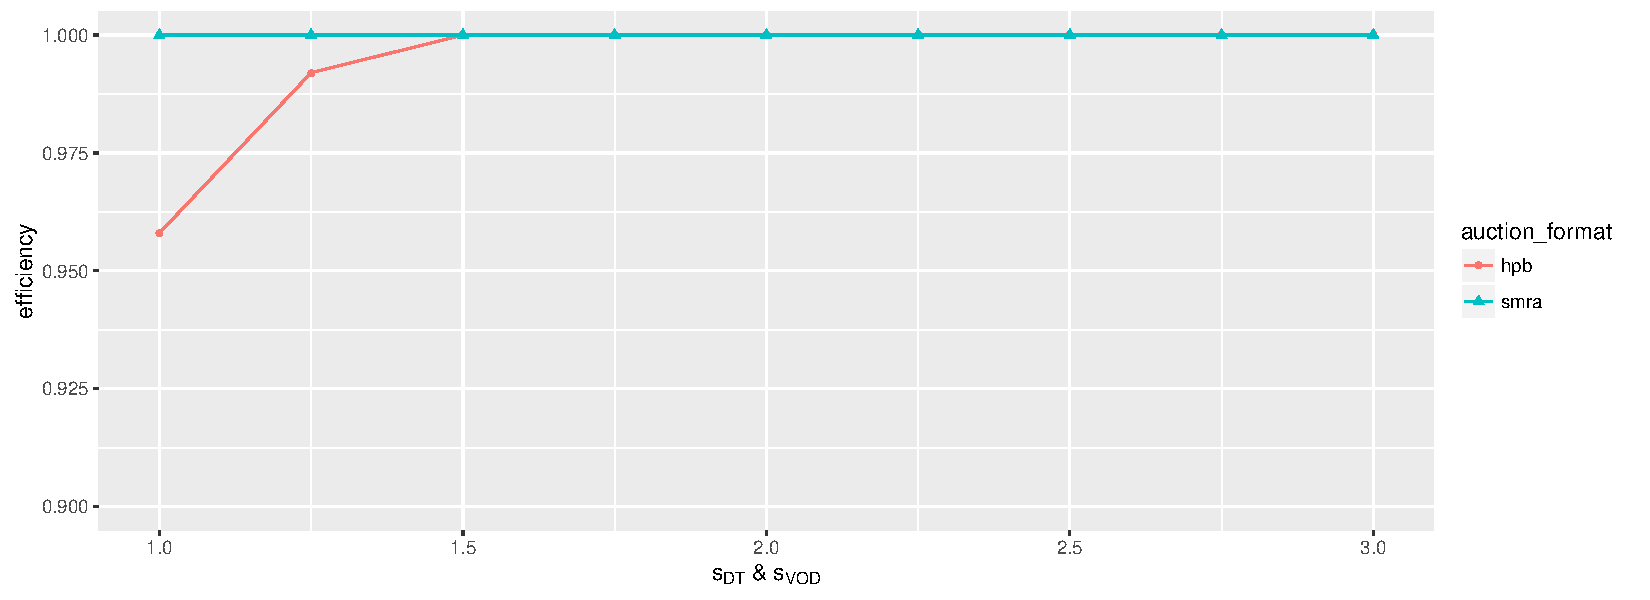
\includegraphics[scale=0.5]{eff_s_both_mov.pdf}
%	\caption{Sensitivity of efficiency against bidder strength $ [s_{DT} = s_{VOD}] $} \label{fig:eff-s-both}
%	
%	\vspace*{\floatsep}
%	
%	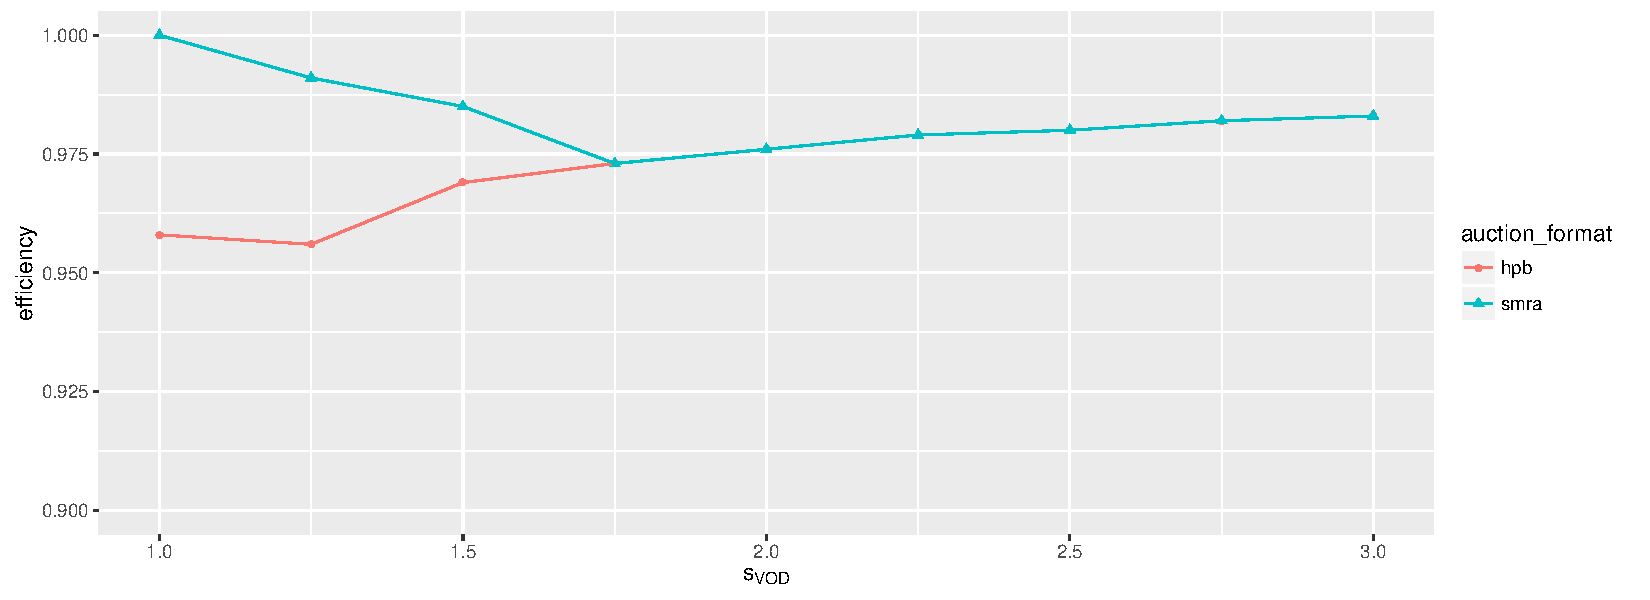
\includegraphics[scale=0.5]{eff_s_singlemov.pdf}
%	\caption{Sensitivity of efficiency with one stronger bidder $ s_{TEF} = s_{DT} = 1 $} \label{fig:eff-s-single}
%\end{figure}
%
%\paragraph{The competition environment.}
%Following the findings from the previous section, I will focus the analysis of the competition environment on the $ H_{competition} $ as maximizing efficiency is a desired property of an auction.

\subsection{Revenue of the Formats}
While reaching an optimal allocation is especially relevant to the participating bidders of an auction, maximizing revenue - to an appropriate level - mostly concerns the auctioneer. As revenue has no upper bound (like efficiency), there is no \textit{perfect} revenue. To analyse the sensitivity of revenue I will at first have a look on the influence of bonus valuations and the hierarchies. Afterwards, I will establish an understanding of the competition environment of the auction formats, meaning the sensitivity towards the distribution of bidder strength.

\paragraph{The influence of bonus valuations and hierarchies.}
\begin{figure}[h]
	\centering
	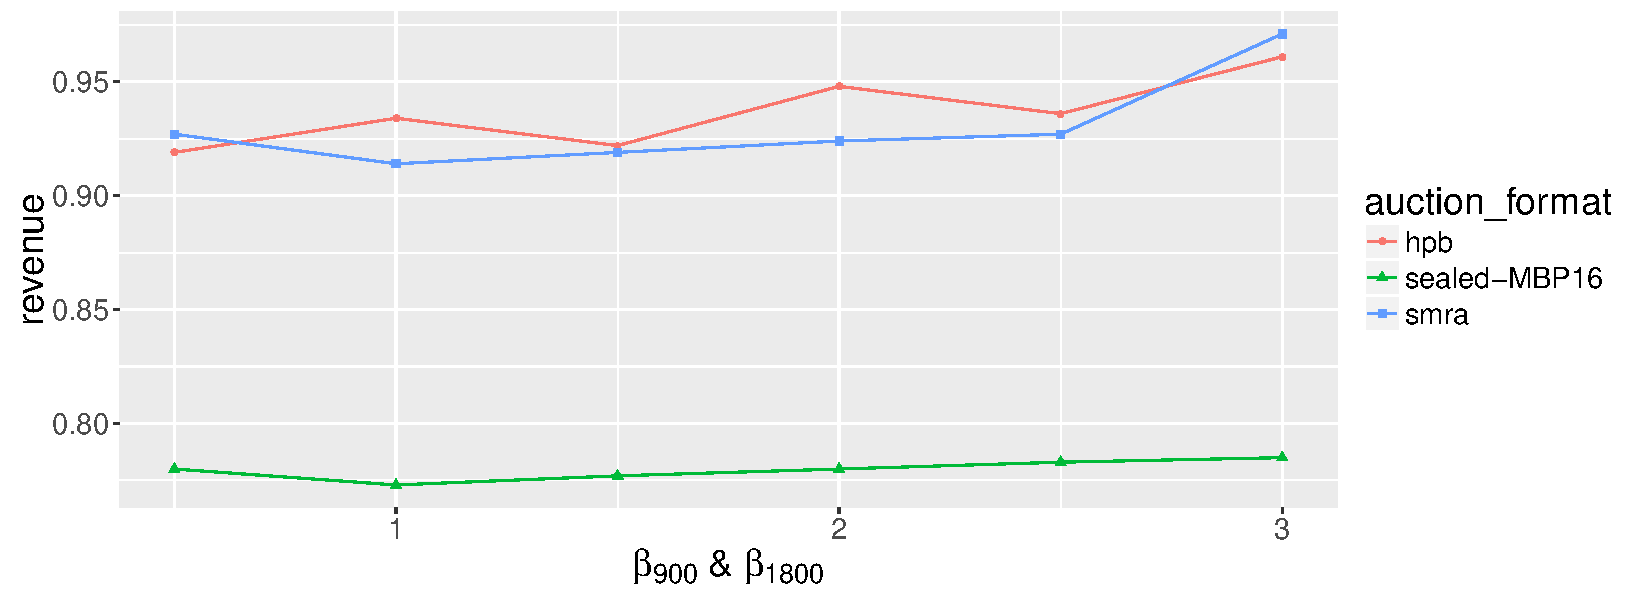
\includegraphics[scale=0.5]{rev_both_beta_mov.pdf}
	\caption{Sensitivity of revenue against $ \beta_{900} = \beta_{1800} $ in $ H_{competition} $} \label{fig:rev-both-beta-mov}
	
	\vspace*{\floatsep}
	
	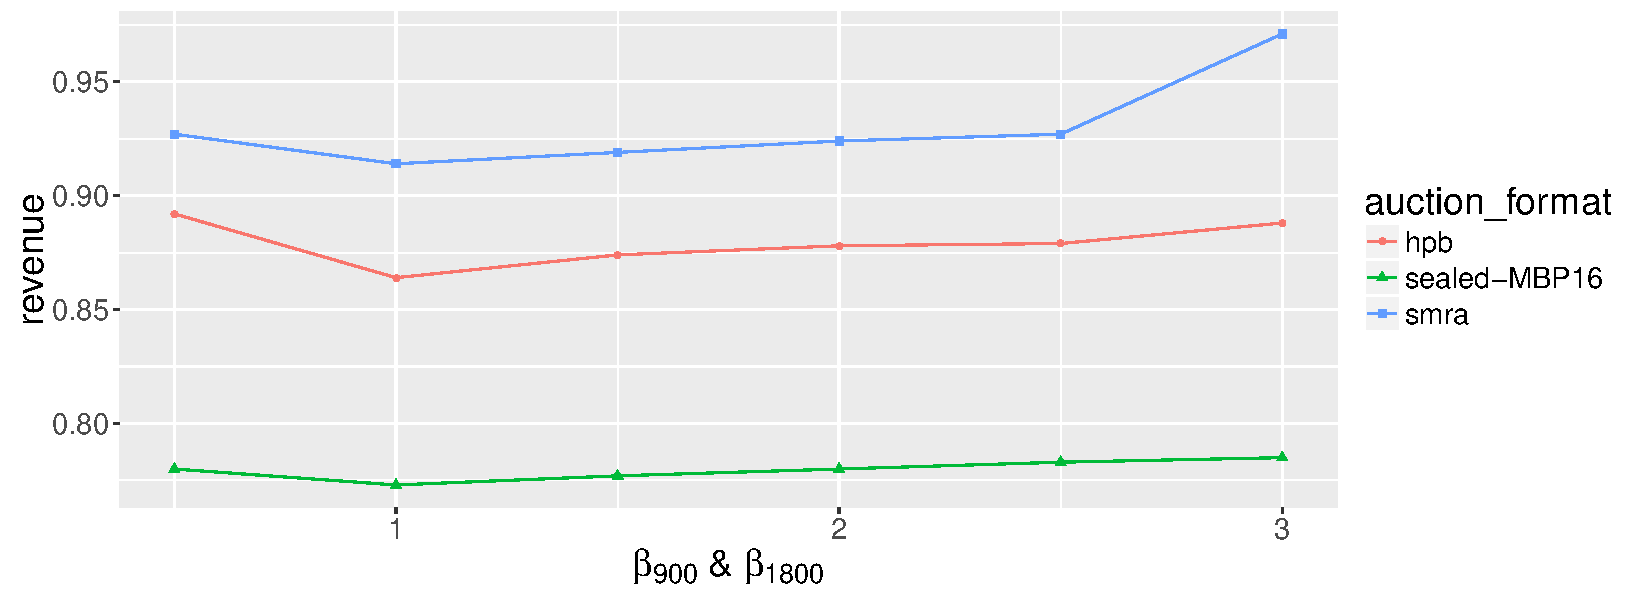
\includegraphics[scale=0.5]{rev_both_beta_mov_VMP.pdf}
	\caption{Sensitivity of revenue against $ \beta_{900} = \beta_{1800} $ in $ H_{vm-prediction} $} \label{fig:rev-both-beta-mov-VMP}
\end{figure}

The general tendency is that $ \beta_{900} \text{ and } \beta_{1800} $ have a positive impact on the development of revenues. With higher bonuses valuations, the overall revenue rises, as can be seen in \autoref{fig:rev-both-beta-mov} and \autoref{fig:hpb-hierarchy-vm-predict}. Interestingly, the effect of the different HPB hierarchies can be observed. 
When using $ H_{competition}  $ in most cases $ \text{HPB} \succ \text{SMRA} $, where the HPB format produced slightly higher revenues in comparison to SMRA. This is contrary to the effect seen in \autoref{fig:hpb-hierarchy-vm-predict}, where $ \text{HPB} \prec \text{SMRA}$ and through beta-space HPB generated prominently lower revenues. Note that in $ H_{vm-prediction} $ two bonuses inducing pre-packaged bundles in the 900 MHz band exist, instead of only one in $ H_{competition}  $. This is an indicator, that HPB might help bidders to coordinate earlier in the auction if the respective hierarchies enable them to, but simultaneously  leading to lower revenue.  Whereas a more competitive HPB hierarchy tends to drive competition and thus revenue.

\paragraph{The competition environment.}
In this section, I will focus on the findings using the  $ H_{competition}  $ hierarchy as it produced the higher efficiency (see \autoref{subsection:eff-formats}) and thus higher social welfare, which I argue to be an optimization goal of an auctioneer.

\begin{figure}[h]
	\centering
	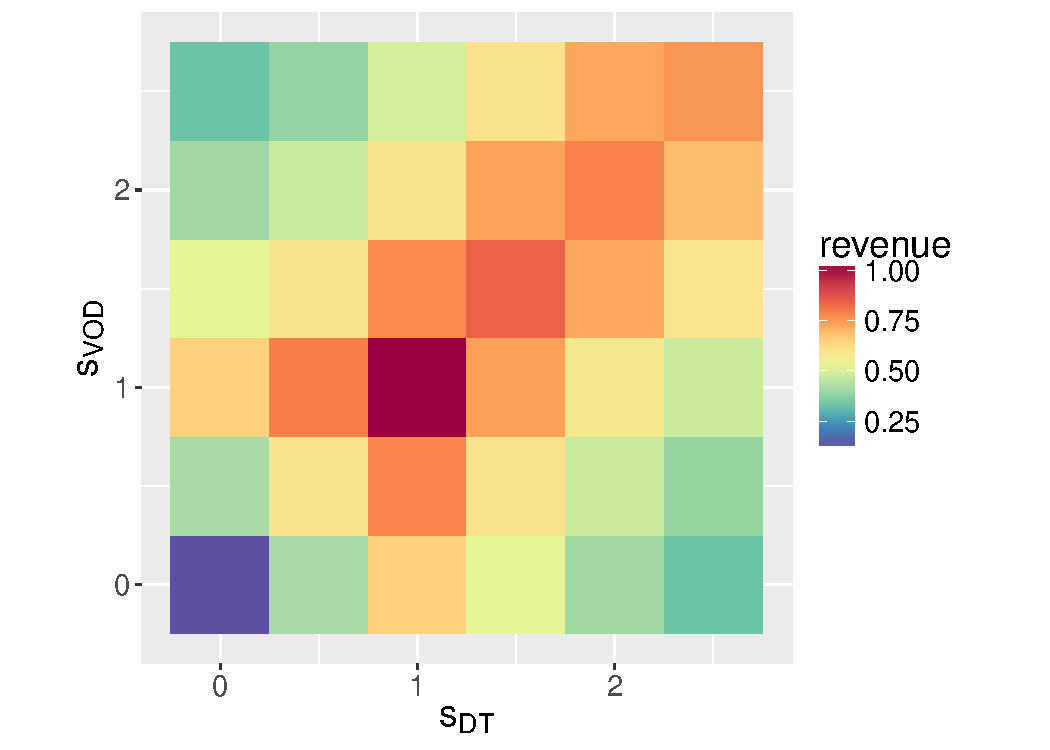
\includegraphics[scale=0.6]{rev_hpb_comp_environment.pdf}
	\caption{Competition environment of HPB with $ H_{competition} \text{ \& } [rev \sim s_{DT}, s_{VOD}] $} \label{fig:rev-hpb-comp-env}
\end{figure}

\autoref{fig:rev-hpb-comp-env} shows the competition environment of the HPB format in the simulation. Each tile shows the revenue generated according to the set-up of the bidder strengths. As can be seen from the figure, when all bidders have the same strength ($ s_{TEF}=s_{DT}=s_{VOD}=1 $) the highest revenues were generated due to the fact, that each bidder had to bid very close to its valuation. In an environment with one very strong bidder, revenues tend to yield much lower level as the strong bidder can much earlier outbid its competitors and thus decrease overall revenue.
As the revenues from both formats were very similar when using the competitive hierarchy (see \autoref{fig:rev-both-beta-mov}), the competition environment also looks very similar. To compare both environments, \autoref{fig:rev-diff-comp-env} depicts the difference between the revenues yielded in HPB and SMRA. The figure suggests, that there is no systematic relation in the superiority or inferiority of an auction format when dealing with different bidder strength environments.

\begin{figure}[b]
	\centering
	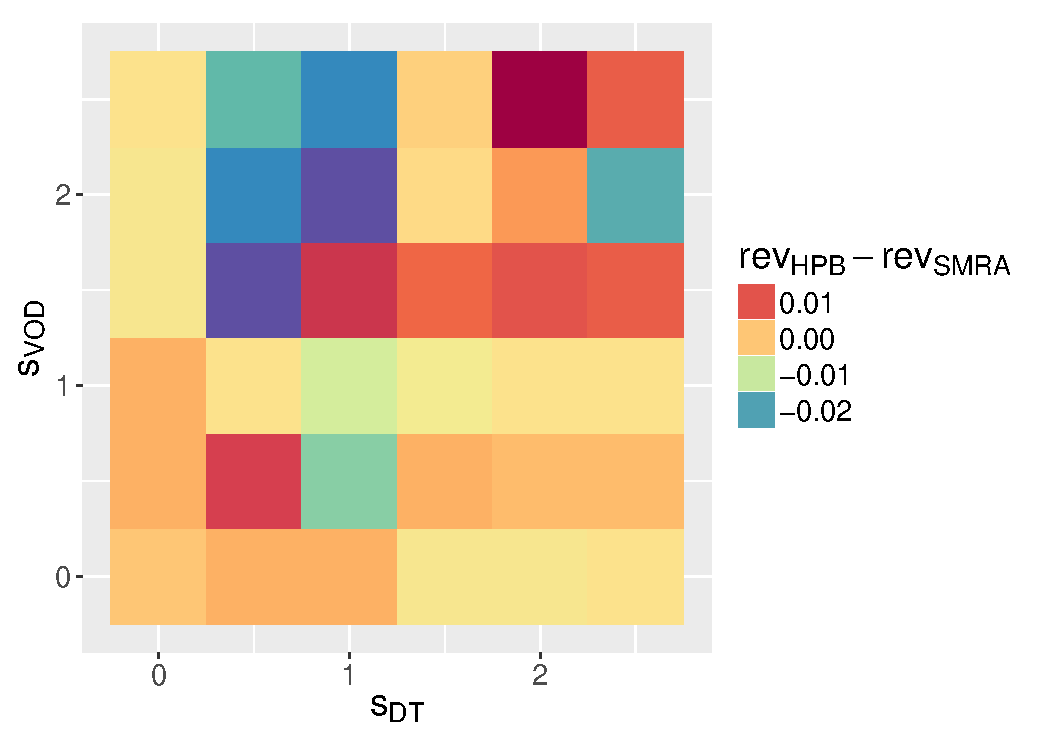
\includegraphics[scale=0.45]{rev_diff.pdf}
	\caption{Competition environment of HPB vs. SMRA $ [rev_{HPB} - rev_{VOD} \sim s_{DT}, s_{VOD}] $} \label{fig:rev-diff-comp-env}
\end{figure}

To compare both formats further, \autoref{fig:rev-s-both} and \autoref{fig:rev-s-single} show the development of revenue in relation to two different bidder strength. As both depict that revenue decreases with increasing bidder strengths, \autoref{fig:rev-s-both} shows that in less unequally distributed bidder environments $ \text{HPB} \succ \text{SMRA} $, where HPB can yield slightly higher revenues even when bidder strengths are high. On the other hand, in an environment where one bidder is much stronger than the other participating bidders, this not only results in much lower revenues, but also slightly lower revenues by the HPB format in comparison to SMRA, even though the difference is marginal.
  

\begin{figure}[h]
	\centering
	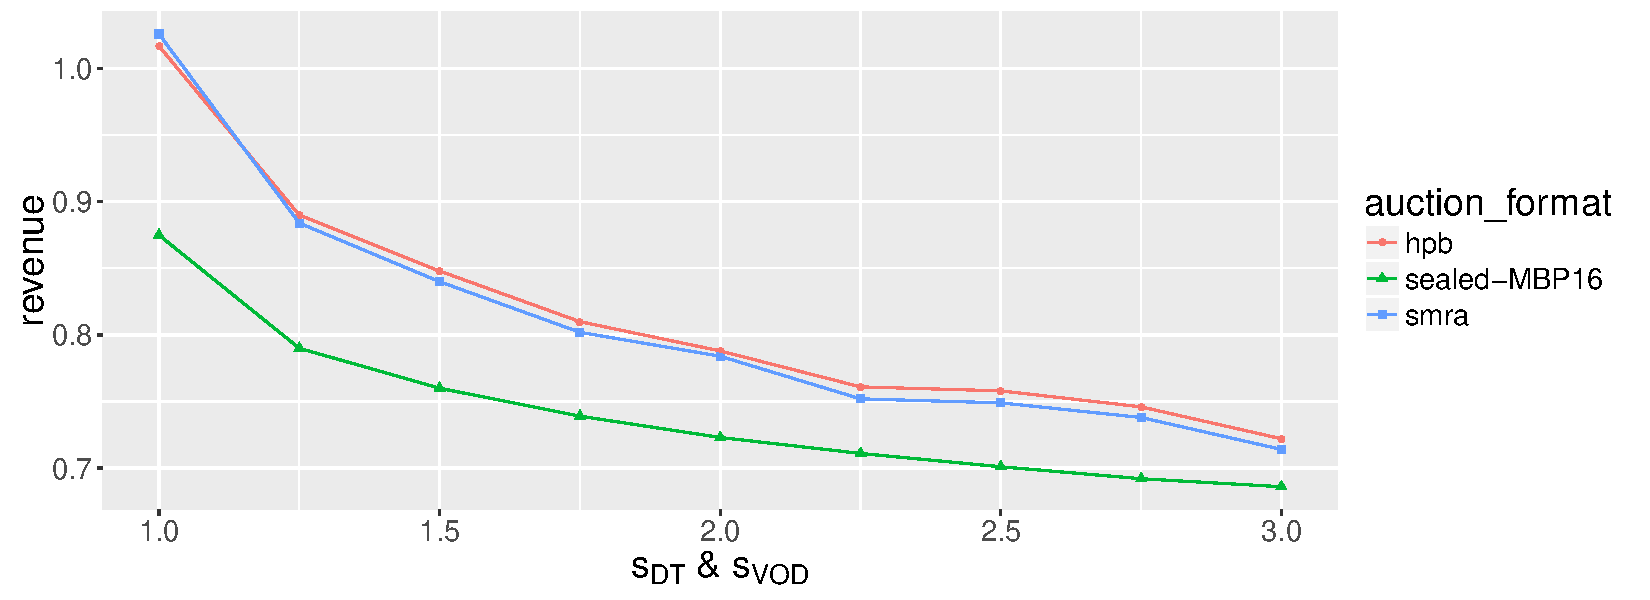
\includegraphics[scale=0.5]{rev_s_bothmov.pdf}
	\caption{Sensitivity of revenue against bidder strength $ [s_{DT} = s_{VOD}] $} \label{fig:rev-s-both}
	
	\vspace*{\floatsep}
	
	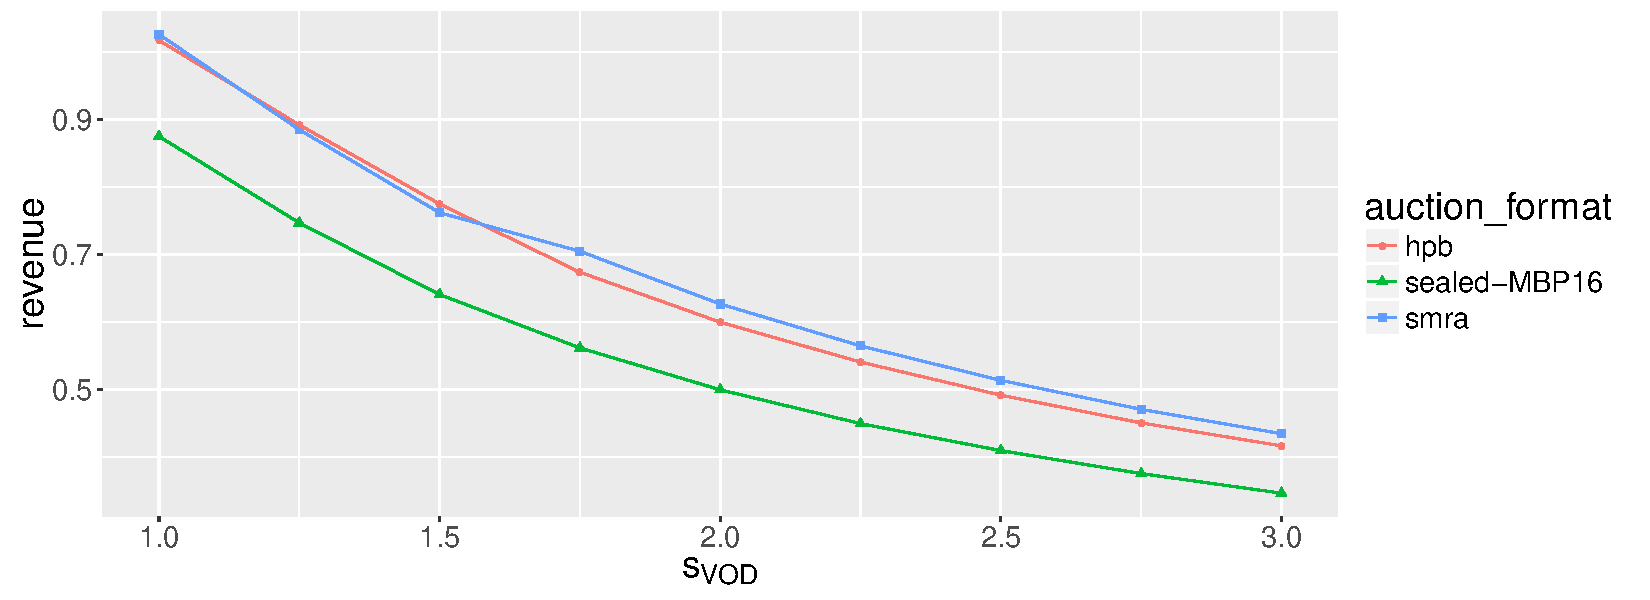
\includegraphics[scale=0.5]{rev_s_singlemov.pdf}
	\caption{Sensitivity of revenue with one stronger bidder $ [s_{TEF} = s_{DT} = 1] $} \label{fig:rev-s-single}
\end{figure}

\subsection{Summary of the Results}
The following table summarises the findings of the simulations, where $ \beta $ means $ \beta_{900} = \beta_{1800} $ and $ s $ means $ s_{DT} = s_{VOD} $.

\begin{table}[h]
	\centering
\begin{tabular}{cc|l|l|}
	\cline{3-4}
	\multicolumn{1}{l}{}                       & \multicolumn{1}{l|}{} & \multicolumn{1}{c|}{\textbf{$\beta$}} & \multicolumn{1}{c|}{\textbf{$s$}} \\ \hline
	\multicolumn{1}{|c|}{\multirow{2}{*}{\textbf{Efficiency}}} & $ H_{competition} $                    & $  HPB \succ SMRA $                         & $ HPB \equiv SMRA $ after $ s= 1.5 
	$                      \\ \cline{2-4} 
	\multicolumn{1}{|c|}{}                     & $ H_{vm-predict} $                 & $ HPB \approx SMRA$                         & $ HPB \prec SMRA $ when $ s > 1 $                      \\ \hline
	\multicolumn{1}{|c|}{\multirow{2}{*}{\textbf{Revenue}}} & $ H_{competition} $                    & $ HPB \succ SMRA $                         & $ HPB \succ SMRA $, rapidly decreasing                      \\ \cline{2-4} 
	\multicolumn{1}{|c|}{}                     & $ H_{vm-predict} $                  & $ HPB \prec SMRA $                         & $ HPB \prec SMRA $                      \\ \hline
\end{tabular}
	\caption{Summary of the findings in the simulations}\label{tbl:sim-results-summary}
\end{table}

From the table it can be seen, that the simulations indicate that HPB might be helpful in enabling bidders to find more efficient overall allocations when choosing an appropriate bidding hierarchy. This improvement came with the reduction of overall revenue as bidder signalling improved. SMRA was superior when a less competitive HPB hierarchy was used, indicating that choosing a suitable hierarchy is key to the success of the auction. 


% BACKUP
%\begin{figure}[h]
%	\centering
%	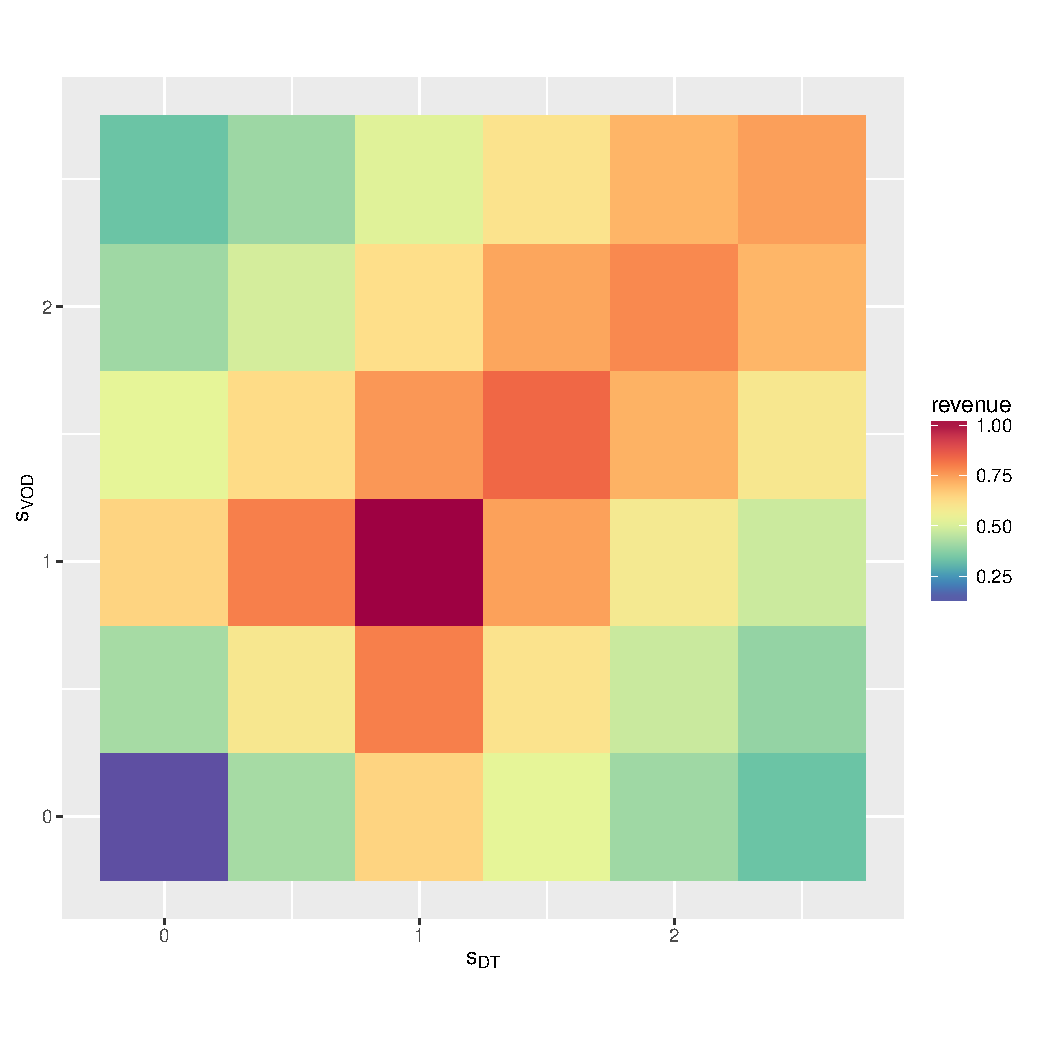
\includegraphics[scale=0.5]{rev_smra_comp_environment.pdf}
%	\caption{Competition environment of SMRA $ [rev \sim s_{DT}, s_{VOD}] $} \label{fig:rev-smra-comp-env}
%	
%	\vspace*{\floatsep}
%	
%	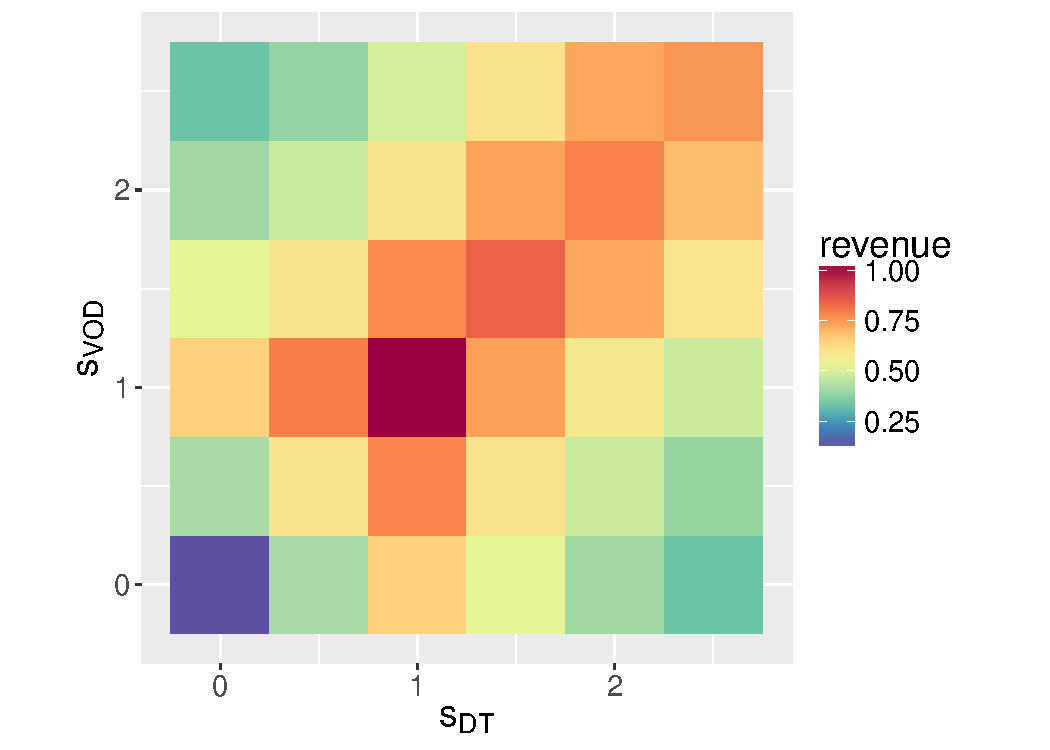
\includegraphics[scale=0.5]{rev_hpb_comp_environment.pdf}
%	\caption{Competition environment of HPB $ [rev \sim s_{DT}, s_{VOD}] $} \label{fig:rev-hpb-comp-env}
%\end{figure}

%\begin{figure}[h]
%	\centering
%	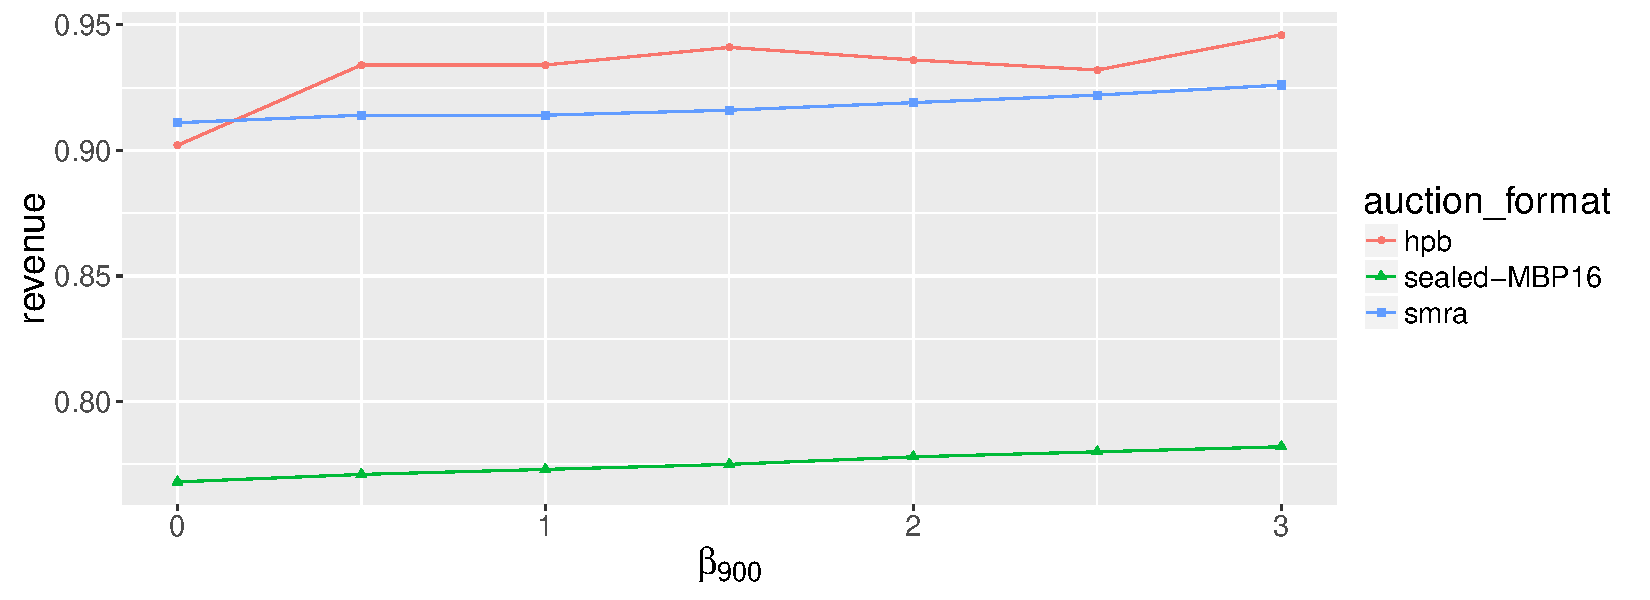
\includegraphics[scale=0.5]{rev_b900mov.pdf}
%	\caption{Sensitivity of revenue against $ \beta_{900} $ with $ \beta_{1800} = 1$} \label{fig:rev-b900-mov}
%	
%	\vspace*{\floatsep}
%	
%	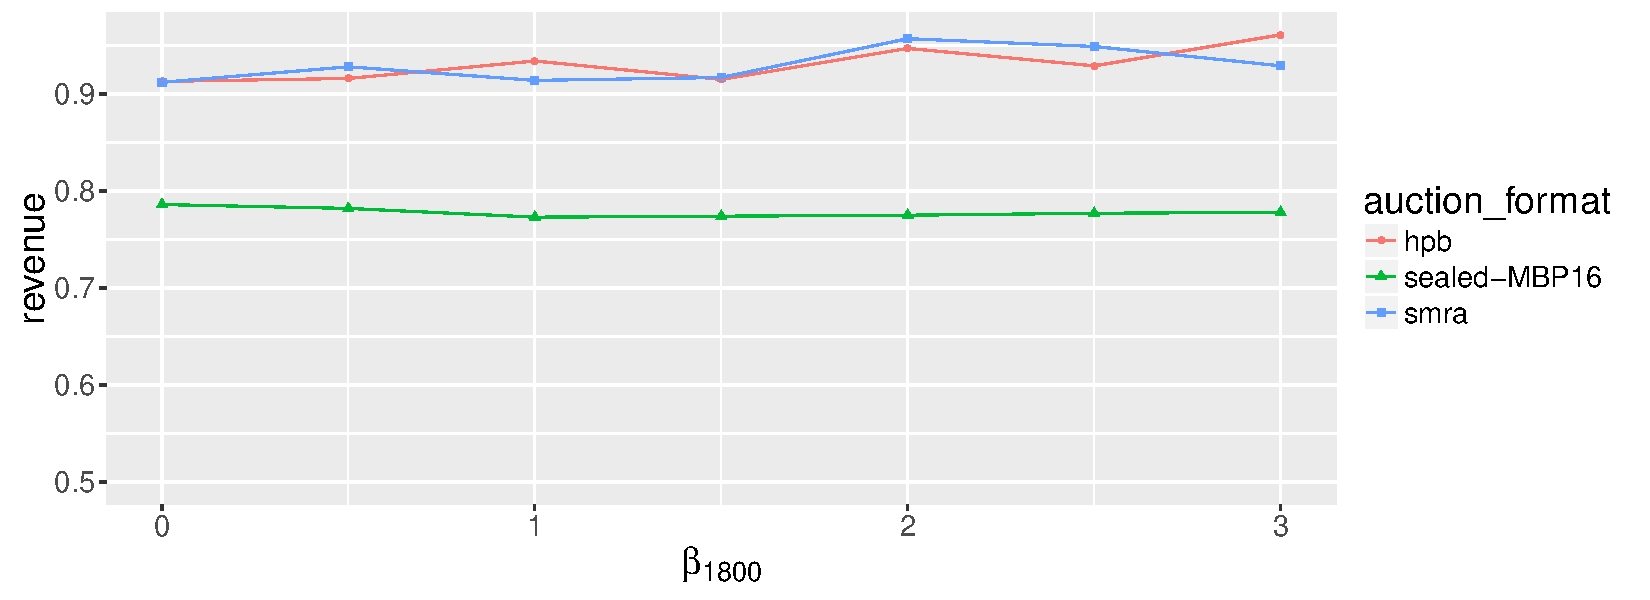
\includegraphics[scale=0.5]{rev_b1800mov.pdf}
%	\caption{Sensitivity of revenue against $ \beta_{1800} $ with $ \beta_{900} = 1$} \label{fig:rev-b1800-mov}
%	
%	\vspace*{\floatsep}
%	
%	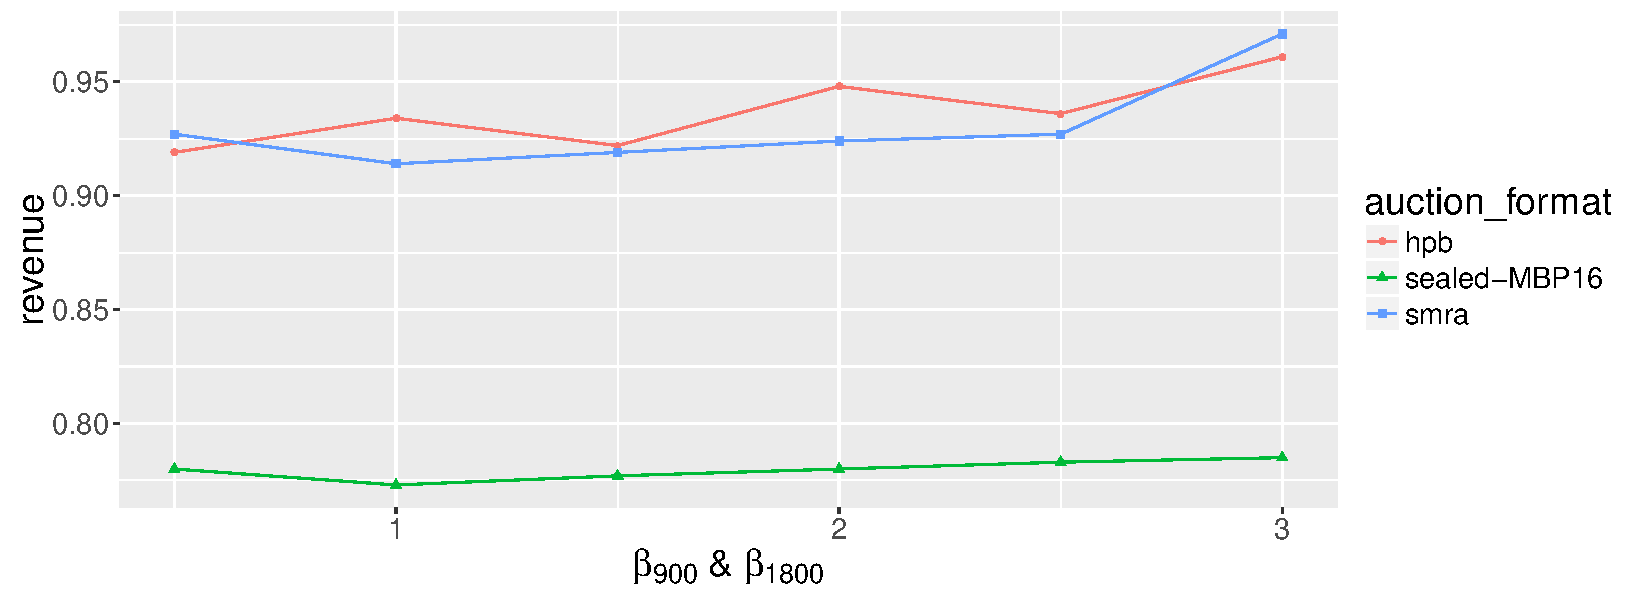
\includegraphics[scale=0.5]{rev_both_beta_mov.pdf}
%	\caption{Sensitivity of revenue against $ \beta_{1800} = \beta_{900} $} \label{fig:rev-both-beta-mov}
%\end{figure}

%\begin{figure}[h]
%	\centering
%	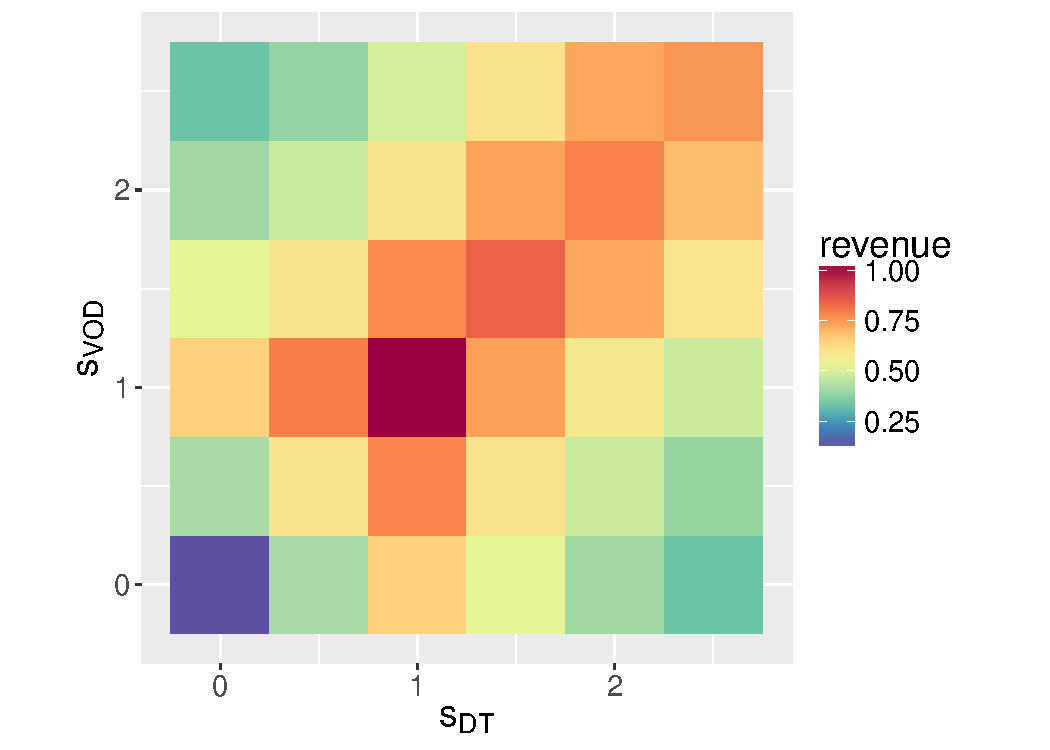
\includegraphics[scale=0.5]{rev_hpb_comp_environment.pdf}
%	\caption{Competition environment of HPB $ [rev \sim s_{DT}, s_{VOD}] $} \label{fig:rev-hpb-comp-env}
%	
%	\vspace*{\floatsep}
%	
%	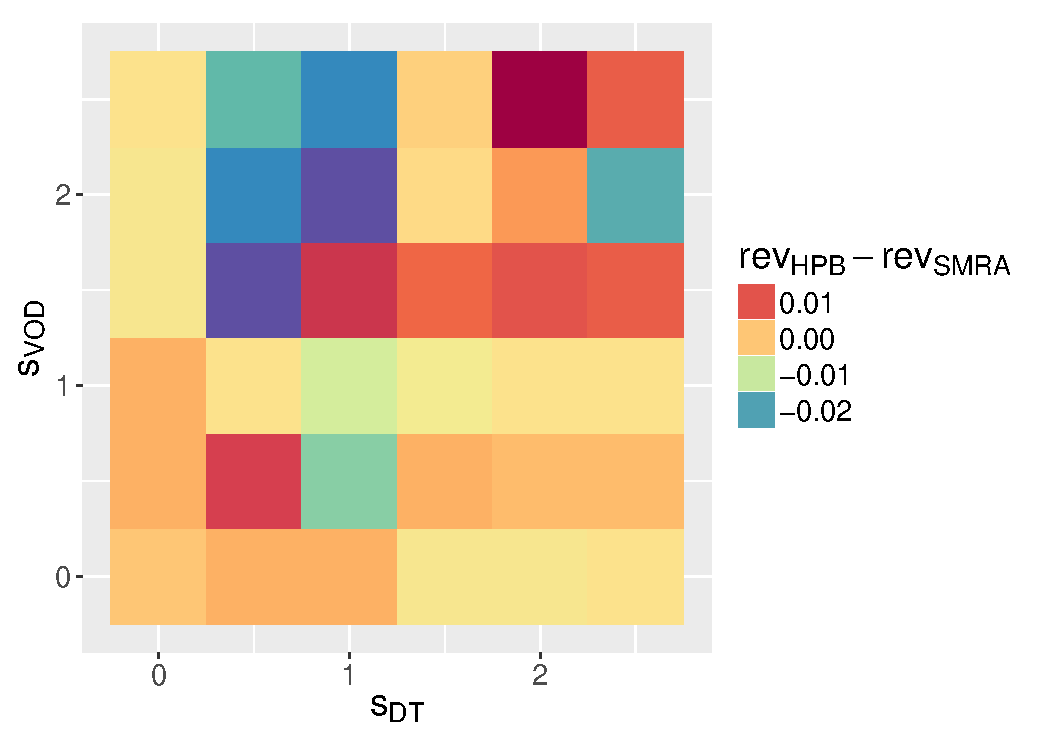
\includegraphics[scale=0.5]{rev_diff.pdf}
%	\caption{Competition environment of HPB vs. SMRA $ [rev_{HPB} - rev_{VOD} \sim s_{DT}, s_{VOD}] $} \label{fig:rev-diff-comp-env}
%\end{figure}

%The impact of the betas are different, because with the caps in the 900 MHz band
%at $ \beta_{1800} = 3 $ are the bonuses that high that it is feasible to buy cheapest four items instead of package (?) and then get the bonus, at $ \beta_{1800} = 2.5 $ it doesnt pay off to do that 
